%!TEX root = ../report.tex
\chapter{Method}
\label{method}

In this chapter the design of the experiment is outlined. The experiment consists of three phases: dataset collection, map segmentation and map stitching. Each of the phases is described in detail below.

\section{Dataset collection}
Three datasets were collected on two recent USARSim maps: the first dataset in a building without smoke, the second two in a larger building. The robot was driven around the map. Care was taken to ensure that the robot visited the same locations a number of times to make the map-stitching method feasible.

Each dataset was recorded, and is available within the code repository\footnote{GitHub code repository \url{http://www.github.com/okke-formsma/slam-confidence/}}.

\begin{figure}[h]
	\centering
	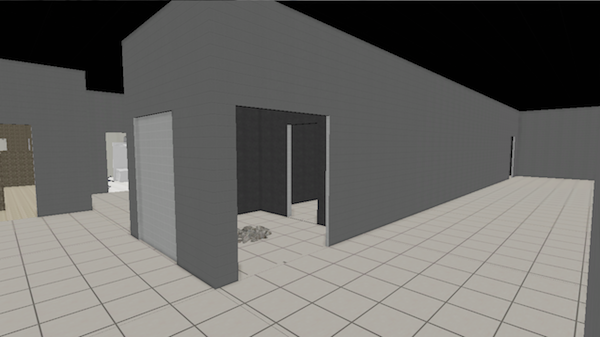
\includegraphics[width=0.9\textwidth]{images/experiment/map1/screenshot.png}
	\label{fig:map1}
	\caption{Screenshot of the simulation environment (Map 1).}
\end{figure}

\section{Map segmentation}
The datasets are processed through the UsarCommander ManifoldSlam implementation. At every timestep the scan matcher runs and saves current position and rotation according to the groundtruth, the inertia sensor and the SLAM algorithm, as well as the correspondence error matrix as discussed in section~\ref{scanmatching}.

After creating the map, three uncertainty metrics are evaluated to decide where the map should be segmented. The three metrics are the determinant of the correspondence error, the trace of the correspondence error and the number of matching scans, as discussed in section~\ref{uncertainty}.

The three metrics are manually examined for each map, as we found no prior research in a good metric for map segmentation. Obvious candidates are the maxima in the determinant and trace measures and minima for the number of matching scans. These values are expected to be highly correlated. The dataset is segmented at the thus acquired uncertainty threshold into consecutive parts. For example, if the map consisted of $100$ timesteps ($0 \ldots 99$) and the uncertainty metrics indicate that the highest uncertainty was at timesteps 11, 25 and 70, the dataset is divided into four segments: $0 \ldots 10$, $11 \ldots 24$, $26 \ldots 69$, and $71 \ldots 99$. A submap is generated for each segment.

\section{Map stitching}
The segments are matched according to the Hough-transform based map stitching method as outlined in chapter~\ref{chapter:hough}. In that chapter it is explained that there may be a number of rotation estimates $\hat \theta$. We will assume in the experiment that the smallest absolute rotation candidate $|\hat \theta|$ will be the most probable. This is based on the observation that the scanmatcher usually does not yield very large rotation errors.

The relative X- and Y-positions of the maps are estimated exactly as explained in the map stitching chapter.

\section{Evaluation}
In line with the exploratory nature of this work the maps will not be evaluated using a groundtruth-metric. Instead, manual assessment of the results will yield a qualitative judgment about the quality of the resulting map. The main concern is whether the resulting map is an improvement upon the map provided by the ManifoldSLAM algorithm.